\chapter{Track Fitting}\label{chapter:KalmanFilter}

\section{Introduction}
Track fitting is the process by which track parameters are determined from a collection of clustered hits. The track parameters include the trajectory, as well as kinematic variables such as the energy or momentum of the particle in question. Track fitting in particle physics is typically performed using a variant of the Kalman filter, which is the optimal estimator for the state of a discrete linear dynamic system.

Originally devised as a noise-reduction and signal filtering technique for communications, the Kalman filter determines optimal estimates of past, present and future states of a linear system based on a series of time-ordered measurements used in conjunction with a statistical model of the system and its measurement errors. It is used extensively for both track and vertex fitting in particle physics, most often in a magnetised detector, where it separates the curvature of a particle due to the magnetic field from the noise introduced by direction changes as a result of multiple scattering.

\section{The Icarus Kalman Filter}
The Icarus~\citep{Amerio2004} experiment presented a Kalman filter~\citep{Fruhwirth1987} which makes statistical use of the distribution of the multiple scattering angle $\theta$ to measure the momentum of a particle in a non-magnetised detector~\citep{Ankowski2006}. The Kalman filter is used to filter out the noise introduced by limited detector resolution. The details of the Icarus algorithm are presented here as an overview of the mechanism of action of the Kalman filter, but also as the basis for the Latte Kalman filter, which aims to perform the same task.

The Kalman filter operates on a discrete set of states, each represented by a state vector $\vec{x}_k$. These states correspond to points on the track, and can in principle be measured anywhere along it. In practice, the track is split into segments of fixed length, and the endpoints of these segments define the set of planes at which the state vector $\vec{x}_k$ is evaluated. 

The track system is described by the linear equation:~\citep{Ankowski2006}
\begin{equation}\label{eqn:kalman_track_system}
    \vec{x}_k^{-} = F_{k-1} \vec{x}_{k-1} + \vec{w}_{k-1}
\end{equation}
Here, $F_{k-1}$ is a matrix defining the propagation of the state vector from plane $k-1$ to plane $k$, $\vec{w}_{k-1}$ is the noise associated with this propagation (which is random, in liquid Argon) and acts to smear the state vector, $\vec{x}_{k-1}$ is the filtered state vector in plane $k-1$, and $\vec{x}_k^{-}$ is the predicted state vector in plane $k$.

The state vector is not usually observed directly; instead, quantities such as the scattering angle are observed, and these are related to quantities in the state vector (such as the particle momentum) through a transformation matrix:
\begin{equation}\label{eqn:kalman_measurement_equation}
    \vec{m}_k = H_k \vec{x}_k + \vec{\epsilon}_k
\end{equation}
where $H_k$ is a matrix transforming a measurement vector $\vec{m}_k$ into a state vector $\vec{x}_k$, and $\vec{\epsilon}_k$ represents measurement noise (errors on the measurements).

The process noise $\vec{w}_k$ and the measurement noise $\vec{\epsilon}_k$ are taken to be unbiased and with finite variance. The covariance matrices are $Q_k$ (for process covariance) and $V_k$ (for measurement covariance). If the process and measurement noise are both random Gaussian variables, the Kalman filter will be the optimal estimator of the system state.

The Kalman filter proceeds through the following three steps, repeated for each new plane $k$ and its corresponding measurement $\vec{m}_k$.

\vspace{1em}\hrule\vspace{1em}
\begin{description}
    \item[1. Prediction:] Given the state vector $\vec{x}_{k-1}$ in plane $k-1$, the prediction step of the Kalman filter estimates the state vector in a future plane $k$, in the absence of noise. The state $\vec{x}_k^{-}$ is the predicted state at plane $k$, using the information contained in all of the state vectors up to $k-1$.
    \begin{equation}\label{eqn:kalman_prediction_step}
        \vec{x}_k^{-} = F_{k-1} \vec{x}_{k-1}
    \end{equation}

    \item[2. Filtering:] Given a predicted state vector $\vec{x}_k^{-}$ (or a suitable initial state), the filtering step determines the present state $\vec{x}_k$ by taking into account the measurements of all previous planes (via the predicted state) and the current plane (via the measurement $\vec{m}_k$). Since the previous measurements are included via their contribution to the state vector, the Kalman filter automatically includes correlations between measurements.
    \begin{equation}\label{eqn:kalman_filtering_step}
        \vec{x}_k = \vec{x}_k^{-} + K_k \left(\vec{m}_k - H_k\vec{x}_k^{-} \right)
    \end{equation}
    where $K_k$ is the Kalman gain matrix, and is related to the covariance of the state vector and the measurement noise.

    \item[3. Smoothing:] When the filter is applied to plane $k+1$, a smoothing step can be used to improve the estimate of the state at plane $k$, taking into account all measurements up to and including $k+1$.
    \begin{equation}
        \vec{x}_k^{n} = \vec{x}_k + A_k \left(\vec{x}_{k+1}^n - \vec{x}_{k+1}^{-}\right)
    \end{equation}
    where $A_k$ is a smoothing gain matrix and $\vec{x}_k^n$ is the filtered state vector after smoothing, for plane $k$.
\end{description}
\vspace{1em}\hrule\vspace{1em}

For particles moving in a non-magnetised detector, the trajectory is split into small track segments, each fitted to a straight line. The state vector $\vec{x}_k$ contains the inverse momentum, coordinates, and track slopes:
\begin{equation}\label{eqn:kalman_state_vector}
    \vec{x}_k = \left( \begin{array}{c} \frac{1}{p} \\ x \\ y \\ \frac{dx}{dz} \\ \frac{dy}{dz} \end{array} \right)
\end{equation}

The transportation matrix $F_k$ provides a straight line extrapolation, with no changes to the track parameters. The energy deposited in a track segment (which can be determined from the charge collected) is subtracted from the momentum estimate in plane $k-1$ to update the momentum estimate in the state vector for plane $k$.

\begin{equation}\label{eqn:kalman_transportation_matrix}
    F_k = \left( \begin{array}{ccccc}
    \frac{1}{1-E_{\mathrm{dep}}/p}  &   0   &   0   &   0       &   0       \\
    0                               &   1   &   0   & \Delta z  &   0       \\
    0                               &   0   &   1   &   0       & \Delta z  \\
    0                               &   0   &   0   &   1       &   0       \\
    0                               &   0   &   0   &   0       &   1
    \end{array} \right)
\end{equation}

The measurement vector includes the coordinates and slopes, but not the inverse momentum. Instead, the angle $\theta_0$ between adjacent track segments at the plane $k$ is used; these angles build up a $\thetarms$ measurement, which is fed to the Kalman filter. Equation \eqref{eqn:kalman_theta_p_relationship} relates this scattering angle to the momentum~\citep{Eidelman2004}.
\begin{equation}\label{eqn:kalman_theta_p_relationship}
    \thetarms = \frac{13.6\MeV}{\beta c p} z \sqrt{\frac{l}{X_0}} \left(1 + 0.038\ln\left[\frac{l}{X_0}\right]\right)
\end{equation}
where $\beta$ is the velocity of the particle, $p$ is its momentum and $z$ is the charge, $X_0$ is the radiation length and $l$ the track segment length. The measurement vector $\vec{m}_k$ is then:
\begin{equation}\label{eqn:kalman_measurement_vector}
    \vec{m}_k = \left( \begin{array}{c} \thetarms \\ x \\ y \\ \frac{dx}{dz} \\ \frac{dy}{dz} \end{array} \right)
\end{equation}

The matrix $H_k$, which relates the measurement and state vectors, is given by:
\begin{equation}\label{eqn:kalman_measurement_matrix}
    H_k = \diag \left( C, 1, 1, 1, 1 \right)
\end{equation}
where $C$ is the constant multiplying $\displaystyle \frac{1}{p}$ in equation \eqref{eqn:kalman_theta_p_relationship}.

Finally, the covariance matrices $Q_k$ (for the system covariance) and $V_k$ (for the measurement covariance) must be taken into account. The Icarus experiment use system covariance matrices from \citep{Wolin1993}, where the covariances for multiple scattering are carefully derived, while the measurements are assumed to be uncorrelated, and the matrix $V$ is diagonal, with each component representing the measurement error.

\section{The Latte Kalman Filter}
The Latte Kalman filter follows closely the formulation used in the Icarus filter. The implementation is based on that present in the SciPy~\citep{SciPy} package for scientific programming in the Python language, with a linear system corresponding to the track fitting mechanism used by Icarus.

The state vector $x_k$ is:
\begin{equation}\label{eqn:kalman_latte_state_vector}
    x_k = \left(\begin{array}{c}
        \frac{1}{p} \\ y \\ z \\ \frac{\Delta y}{\Delta x} \\ \frac{\Delta z}{\Delta x}
    \end{array}\right)
\end{equation}

The measurement vector is identical to the state vector, except for the scattering angle $\thetarms$ in place of the inverse momentum:
\begin{equation}\label{eqn:kalman_latte_measurement_vector}
    x_k = \left(\begin{array}{c}
        \thetarms \\ y \\ z \\ \frac{\Delta y}{\Delta x} \\ \frac{\Delta z}{\Delta x}
    \end{array}\right)
\end{equation}


The process covariance matrix $Q$ is a $5\times 5$ matrix defined as:~\citep{Wolin1993}
\begin{equation}\label{eqn:kalman_process_covariance_matrix}
    Q = \left(
    \begin{array}{ccccc}

        \left(\frac{0.01}{p}\right)^2 &                 0 &                 0 &                0 &                0 \\
                                    0 & \Delta x^2 P_{33} & \Delta x^2 P_{34} & -\Delta x P_{33} & -\Delta x P_{34} \\
                                    0 & \Delta x^2 P_{34} & \Delta x^2 P_{44} & -\Delta x P_{34} & -\Delta x P_{44} \\
                                    0 & -\Delta x P_{33}  & -\Delta x P_{34}  & P_{33}           & P_{34}           \\
                                    0 & -\Delta x P_{34}  & -\Delta x P_{44}  & P_{34}           & P_{44}           

    \end{array}
    \right)
\end{equation}
where $p$ is the momentum at that step, $\Delta x$ is the segment length in the $x$ direction, and
\begin{align*}
    P_{33} &= \theta (1 + S_y^2)(1 + S_y^2 + S_z^2) \\
    P_{34} &= \theta S_y S_z(1 + S_y^2 + S_z^2) \\
    P_{44} &= \theta (1 + S_z^2)(1 + S_y^2 + S_z^2)
\end{align*}
where $\theta$ is the scattering angle, and $\displaystyle S_y=\frac{\Delta y}{\Delta x}$ and $\displaystyle S_z = \frac{\Delta z}{\Delta x}$ are the slopes in $y$ and $z$.

The measurement covariance matrix is diagonal, with components representing the measurement uncertainties on the values of $\theta$, $y$, $z$, $\displaystyle\frac{\Delta y}{\Delta x}$ and $\displaystyle\frac{\Delta z}{\Delta x}$ respectively:
\begin{equation}\label{eqn:kalman_measurement_covariance_matrix}
    V = \diag \left( 1\times10^{-4}, ~ 0.1, ~ 0.1, ~ 1\times10^{-3}, ~ 1\times10^{-3} \right)
\end{equation}

Tracks are split into segments of length $L$ (in $\mm$), with the Kalman filter applied to the points between two segments, and using the slopes of those segments to determine the scattering angle $\theta$ and the distribution of those angles to establish $\thetarms$. The segment lengths are chosen to be a multiple of the radius $R$ (in $\mm$) used for a charge smoothing process which reduces the total number of hits in the track, replacing groups of hits with a single charge-weighted hit. The track momentum is taken from the first component of the state vector after running along the entire track.

\section{Tuning the Kalman Filter}\label{sec:kalman-tuning}
The majority of parameters for the Kalman Filter are fixed by either the process itself (the description of multiple scattering that relates scattering angles to momenta) or by the measurement errors. The remaining free parameters are $R$ and $L$, the charge smoothing radius and segment length, respectively.

A sample of single muon events was generated using the Lamu simulation, producing 100 muons at each energy in the range $100$ to $5000\MeV$ in $100\MeV$ increments. The muon hits from these events were processed using the Kalman filter, and the resulting momentum measurements recorded. The true momentum $p$ is related to the initial kinetic energy $T$ by:\footnote{$E^2 = p^2+m^2$ and $E = T + m$, so $p^2 + m^2 = T^2 + m^2 + 2\,T m$ and the result above can be obtained by a cancellation of $m^2$ followed by the square root operator. This of course assumes natural units, i.e. $c=1$.}
\begin{equation}\label{eqn:momentum-kinetic-energy-relationship}
p = \sqrt{T^2 + 2\,T m}
\end{equation}
where $m$ is the mass of the muon, $105.6583715\MeV$~\citep{PDG2011}.

The segment length was initially chosen to be six times the charge smoothing radius, and the radius varied between $20.1\mm$ and $50.1\mm$. Figure \ref{fig:kalman-mu-momentum-charge-radius-variations} shows the resulting measurements, represented by the mean reconstructed momentum as a function of the true momentum. Smaller smoothing radii ($20.1\mm$) give smaller standard deviation in the results, especially at high momentum, while the mean values are closer to the true momentum for larger smoothing radii of $30.1\mm$ to $40.1\mm$. The distributions of residuals (defined as $p_{\mathrm{true}} - p_{\mathrm{recon}}$) are presented in figure \ref{fig:kalman-residuals} for each of the radii considered here. At momenta over approximately $500\MeV$, the Kalman filter underestimates the momentum when used with short ($20.1\mm$ and $30.1\mm$) segment lengths, but overestimates it for larger segment lengths. As the segment length increases, the range of momentum estimates also increases (both in the positive and negative directions). The Kalman filter in this configuration does not, therefore, provide reliable estimates of momentum.

\begin{figure}
\centering
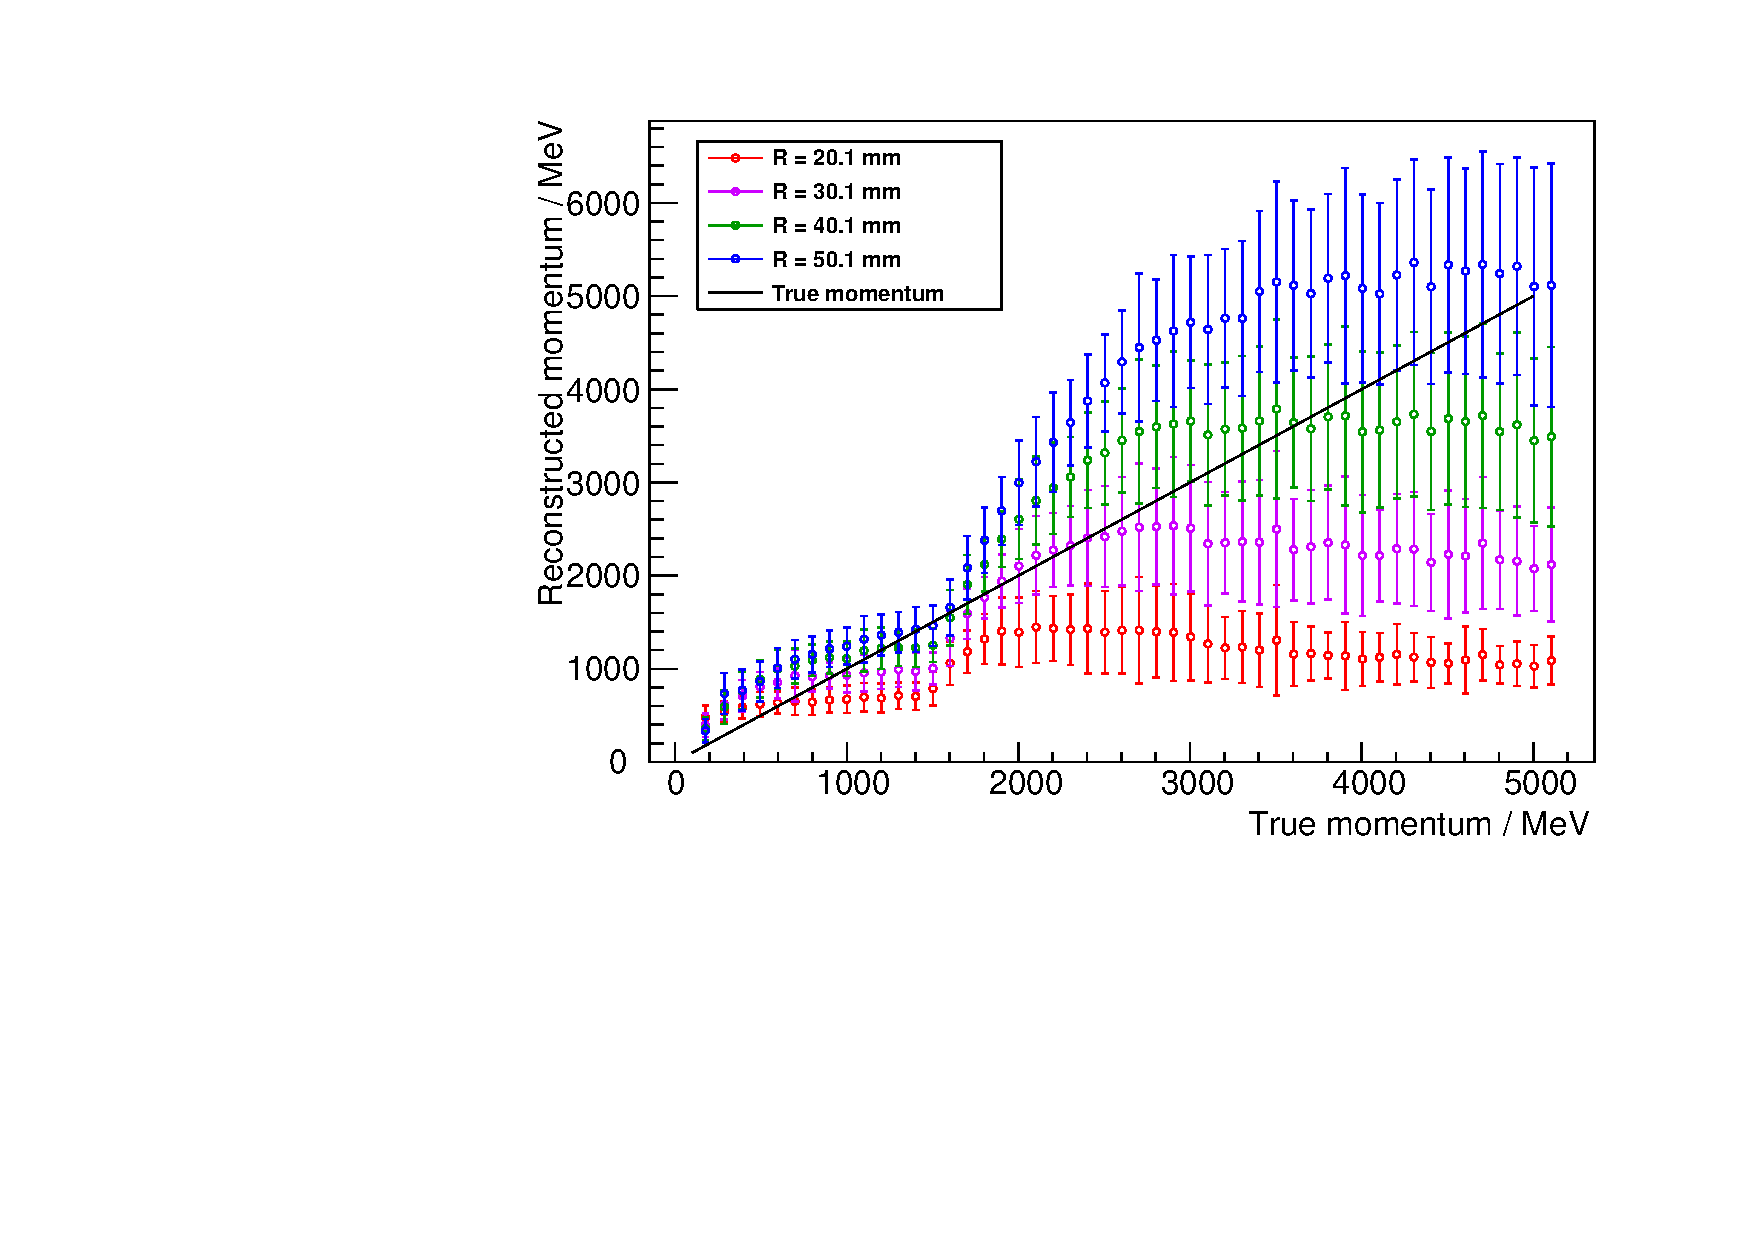
\includegraphics[angle=-90,width=\textwidth]{chapters/trackfitting_images/kalman-mu-momentum-reconstruction}
\caption[Reconstructed momenta for various Kalman filter parameters]{\label{fig:kalman-mu-momentum-charge-radius-variations}The mean and standard deviation of reconstructed momenta as a function of the true momenta of single muons after application of the Kalman filter, for four values of the charge smoothing radius $R$ (and consequently the segment length $L=6R$).}
\end{figure}

\begin{figure}
\centering

\subfigure[$R=20.1\mm$]{
    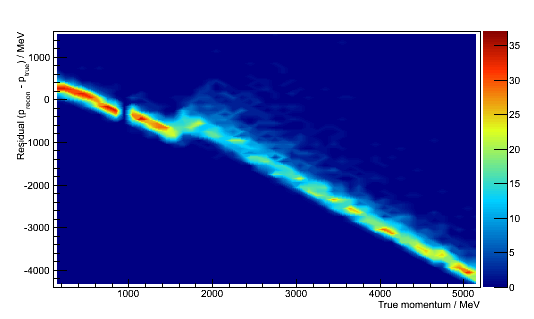
\includegraphics[angle=90,width=0.4\textwidth]{chapters/trackfitting_images/r20}
    \label{fig:kalman-residuals-20}
}
\subfigure[$R=30.1\mm$]{
    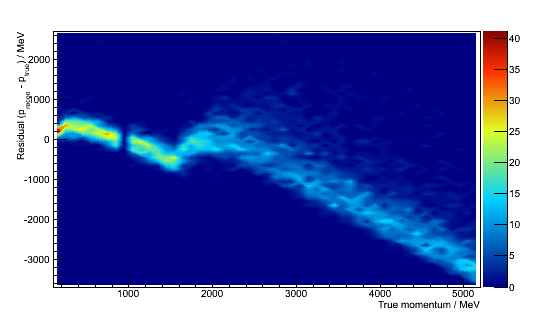
\includegraphics[angle=90,width=0.4\textwidth]{chapters/trackfitting_images/r30}
    \label{fig:kalman-residuals-30}
}
\subfigure[$R=40.1\mm$]{
    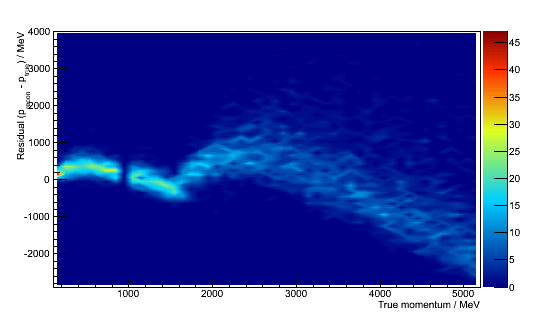
\includegraphics[angle=90,width=0.4\textwidth]{chapters/trackfitting_images/r40}
    \label{fig:kalman-residuals-40}
}
\subfigure[$R=50.1\mm$]{
    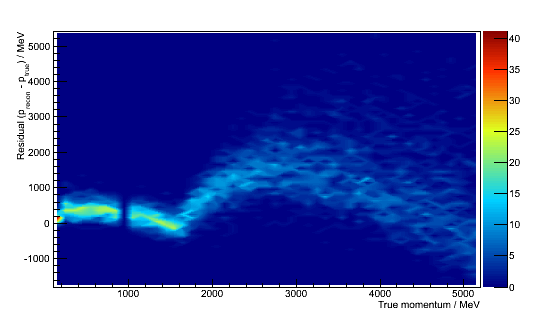
\includegraphics[angle=90,width=0.4\textwidth]{chapters/trackfitting_images/r50}
    \label{fig:kalman-residuals-50}
}

\caption[Momentum residuals for various Kalman filter parameters]{\label{fig:kalman-residuals}Residuals (reconstructed momentum minus true momentum) for the Kalman filter with different values of the charge smoothing radius $R$, and therefore of the segment length $L=6R$. The gaps around $1000\MeV$ are due to the $100\MeV$ bin width used. See text for discussion.}
\end{figure}

\section{Momentum Measurements of CCQE $\mu$ tracks}
In the tuning study of chapter \ref{sec:kalman-tuning}, muons of a fixed kinetic energy (and, therefore, momentum) were used to attempt to validate the Kalman filter algorithm and the choice of parameters. The results indicate that for a $50.1\mm$ charge smoothing radius, and choosing segment lengths six times that radius, the mean momentum measurement is close to the true momentum, but the range of measurements is extremely large.

In this section, the Kalman filter is applied to hits produced by the muon generated from charged current $\nu_\mu$ interactions on Argon nuclei, resulting in $\ccqe$ final states. Two neutrino energies are considered; $E_\nu = 770\MeV$ (1000 events) and $E_\nu = 4.5\GeV$ ($10^4$ events). For the high energy data, the detector simulation was expanded to a cylinder of radius $25\metre$ and height $50\metre$. Muons produced in these interactions have a range of energies and momenta, as well as a distribution of trajectories determined by Genie from the interaction physics models. The true momentum, stored in the Genie event data, was extracted for comparison against the measurements from the Kalman filter. Figure \ref{fig:kalman-ccqe-low} shows the two distributions for the $770\MeV$ neutrinos, and figure \ref{fig:kalman-ccqe-high} shows the distributions for the $4.5\GeV$ neutrinos.

\begin{figure}
\centering
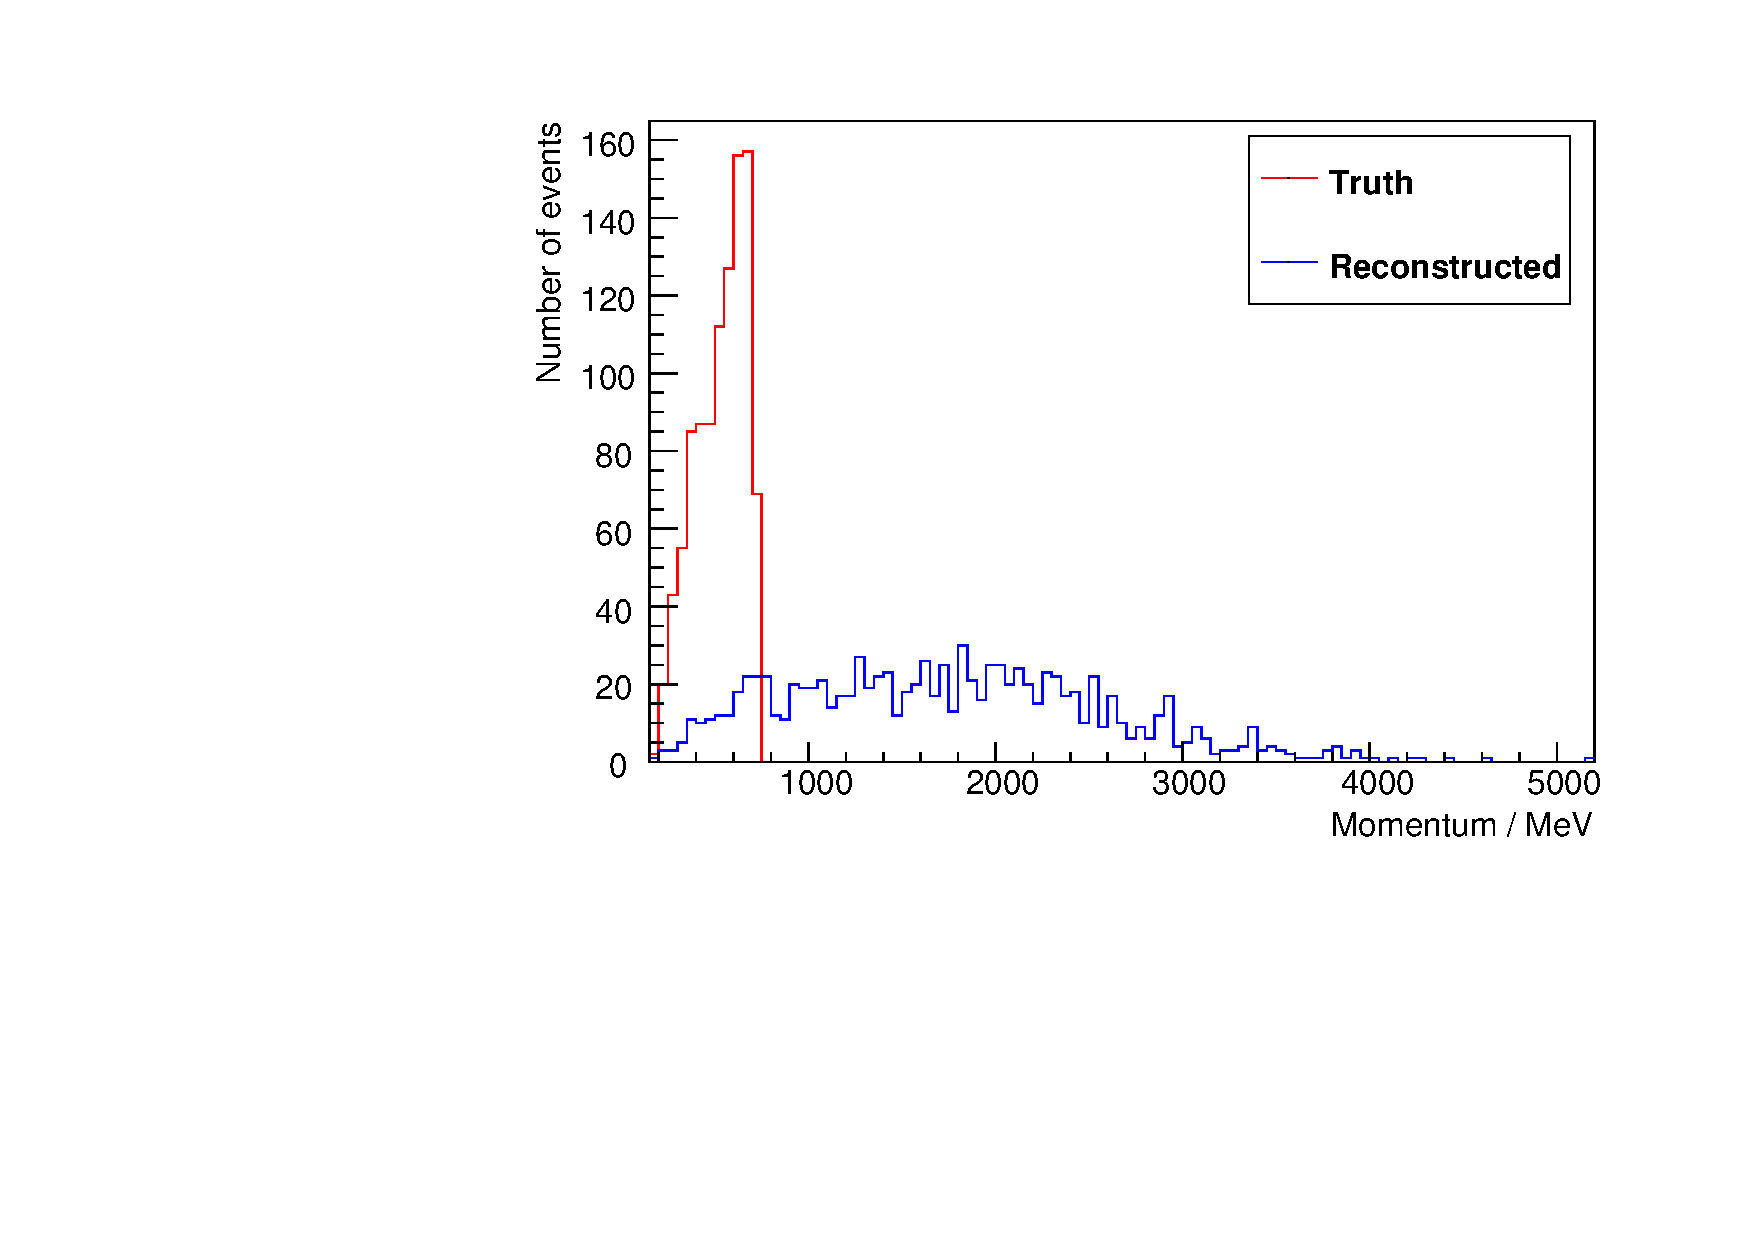
\includegraphics[angle=-90,width=\textwidth]{chapters/trackfitting_images/kalman-ccqe-low}
\caption[True and reconstructed muon momentum distributions at $770\MeV$]{\label{fig:kalman-ccqe-low}Distribution of momenta for muons produced in a charged current low energy $\nu_\mu$ interaction at $770\MeV$ resulting in a $\ccqe$ (only) final state (in red). The distribution of reconstructed momenta (in blue) is from the output of the Kalman filter applied to 1000 such events. The distribution produced by the Kalman filter does not match the true distribution, being both flatter and shifted to higher momentum. The filter therefore overestimates (in general) the momentum of these muons (represented by the shift to higher momentum), but not in a consistent manner (represented by the flatness).}
\end{figure}

\begin{figure}
\centering
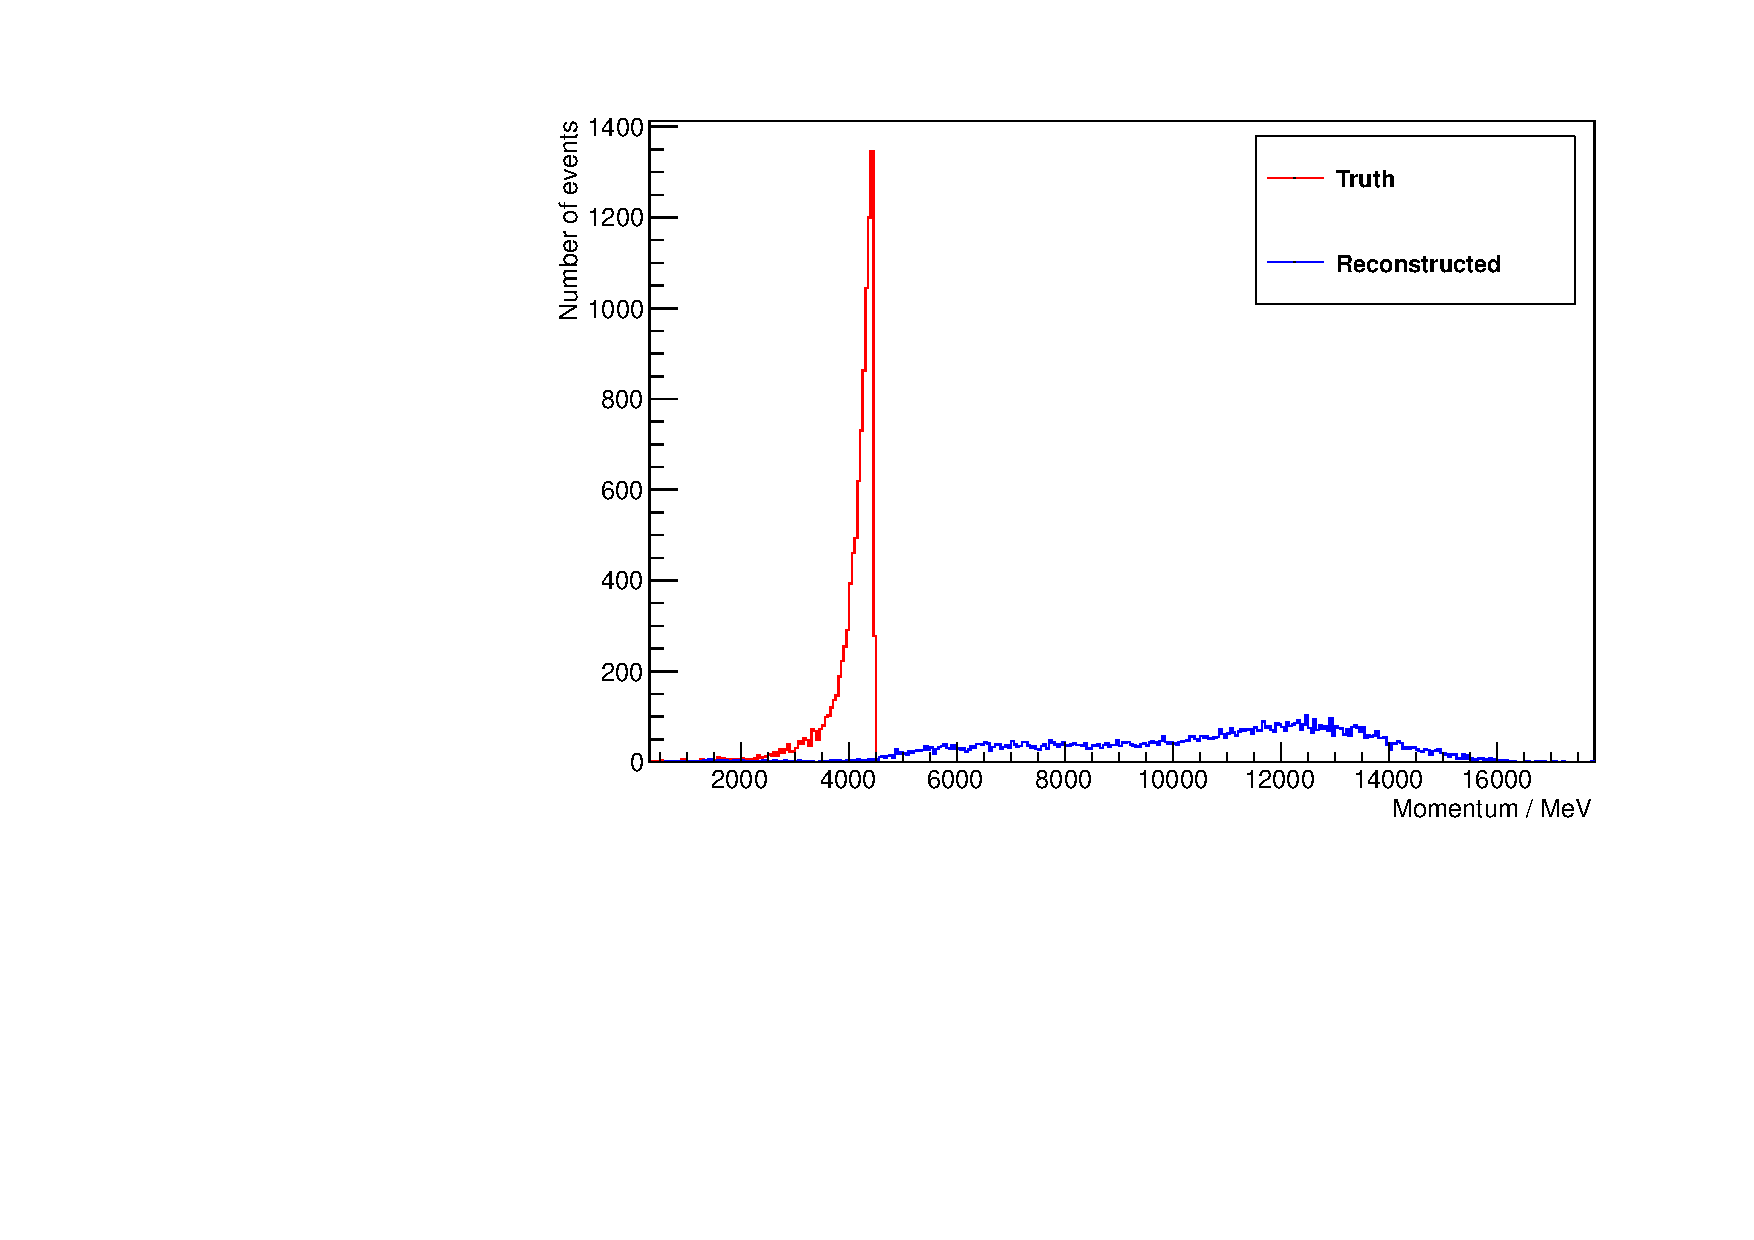
\includegraphics[angle=-90,width=\textwidth]{chapters/trackfitting_images/kalman-ccqe-high}
\caption[True and reconstructed muon momentum distributions at $4.5\GeV$]{\label{fig:kalman-ccqe-high}Distribution of momenta for muons produced in a charged current high energy $\nu_\mu$ interaction at $4.5\GeV$ resulting in a $\ccqe$ (only) final state (in red). The distribution of reconstructed momenta (in blue) is from the output of the Kalman filter applied to $10^4$ such events. As for the low energy distribution, the Kalman filter produces overestimates of the muon momentum, though the effect is much more pronounced here.}
\end{figure}

The Kalman filter overestimates the momentum in both the low energy and high energy neutrinos, though the effect is much more pronounced at high energy. Since the method of estimating momentum through the Kalman filter relies on measurements of the multiple scattering angle, these observations correspond to an underestimate of the angle. The angle is more likely to be underestimated at high energy since the effect of scattering is smaller there.

\subsection{Constrained Momentum Measurements}
The data in figure \ref{fig:kalman-mu-momentum-charge-radius-variations} implies that an energy (momentum) dependent choice of the smoothing radius may provide better results, but it is not possible to use this in a general purpose reconstruction algorithm, since the momentum is not known in advance. Indeed, the purpose of applying the Kalman filter is to obtain an estimate of this momentum. The distributions of reconstructed momenta for $E_\nu = 770\MeV$ and $E_\nu = 4.5\GeV$ extend far beyond the energy of the parent neutrino; a situation which is unphysical. Since the maximum possible neutrino energy (i.e. the beam energy) can be known in advance, it is possible to run the Kalman filter in a configuration that enforces constraints on the momentum estimate at each step.

In figure \ref{fig:kalman-constrained-ccqe-770} the distributions of true and reconstructed momenta are shown for $770\MeV$ CCQE interactions resulting in $\mu + p$ final states, where the Kalman filter was constrained such that at each step, the estimated momentum $|\vec{p}|$ must lie between $0\MeV$ and $770\MeV$. The residuals (i.e. the reconstructed momentum minus the true momentum) for this reconstruction are shown in figure \ref{fig:kalman-constrained-ccqe-770-residuals}; the residual is calculated per muon, and a value close to zero indicates compatibility between the true momentum and the reconstructed momentum estimate.

Both plots demonstrate that even with the momentum constrained, the reconstructed values do not agree with the truth. The constraint serves only to truncate all momenta with estimates that would exceed the maximum, resulting in a large peak at the maximum value allowed. From the residuals plot, it is clear that the Kalman filter still over-estimates the momentum of a given track (that is, there are more events on the positive side of the zero point than on the negative side), and that only 5 events out of 1000 have a residual of zero, indicating perfect reconstruction. Many more events have large residuals of over $200\MeV$, and these momentum estimates are not suitable for use in later stages of a general purpose reconstruction chain.

\begin{figure}
    \centering
    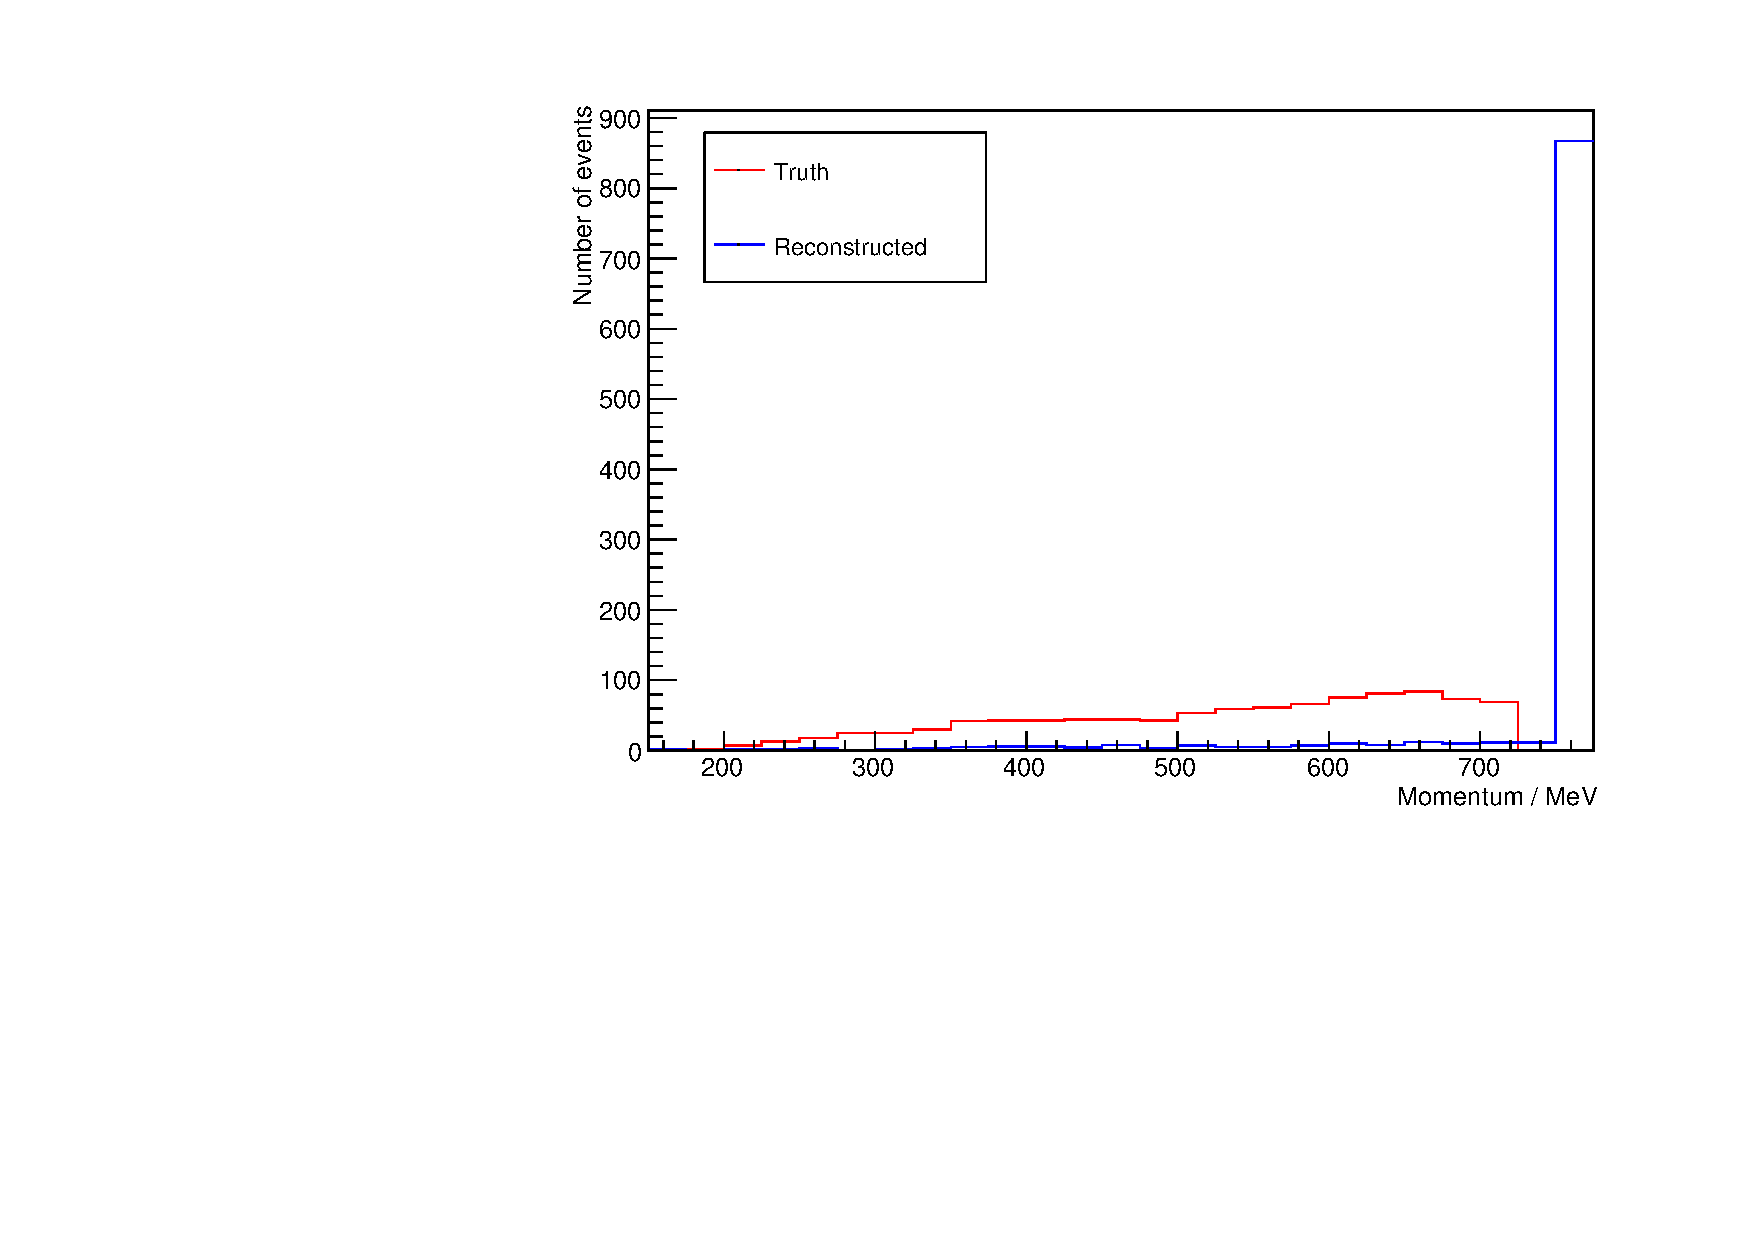
\includegraphics[angle=-90,width=\textwidth]{chapters/trackfitting_images/kalman-ccqe-low-constrained}
    \caption[True and reconstructed muon momentum distributions at $770\MeV$ (constrained)]{\label{fig:kalman-constrained-ccqe-770}Distribution of momenta for muons produced in a charged current $\nu_\mu$ interaction at $770\MeV$ resulting in a $\ccqe$ (only) final state (in red). The distribution of reconstructed momenta (in blue) is from the output of the Kalman filter applied to $10^3$ such events, with the momentum estimate at each step constrained such that $0 \le |\vec{p}| \le 770\MeV$. The distributions do not agree, and the highest momentum bin contains almost all of the reconstructed events.}
\end{figure}

\begin{figure}
    \centering
    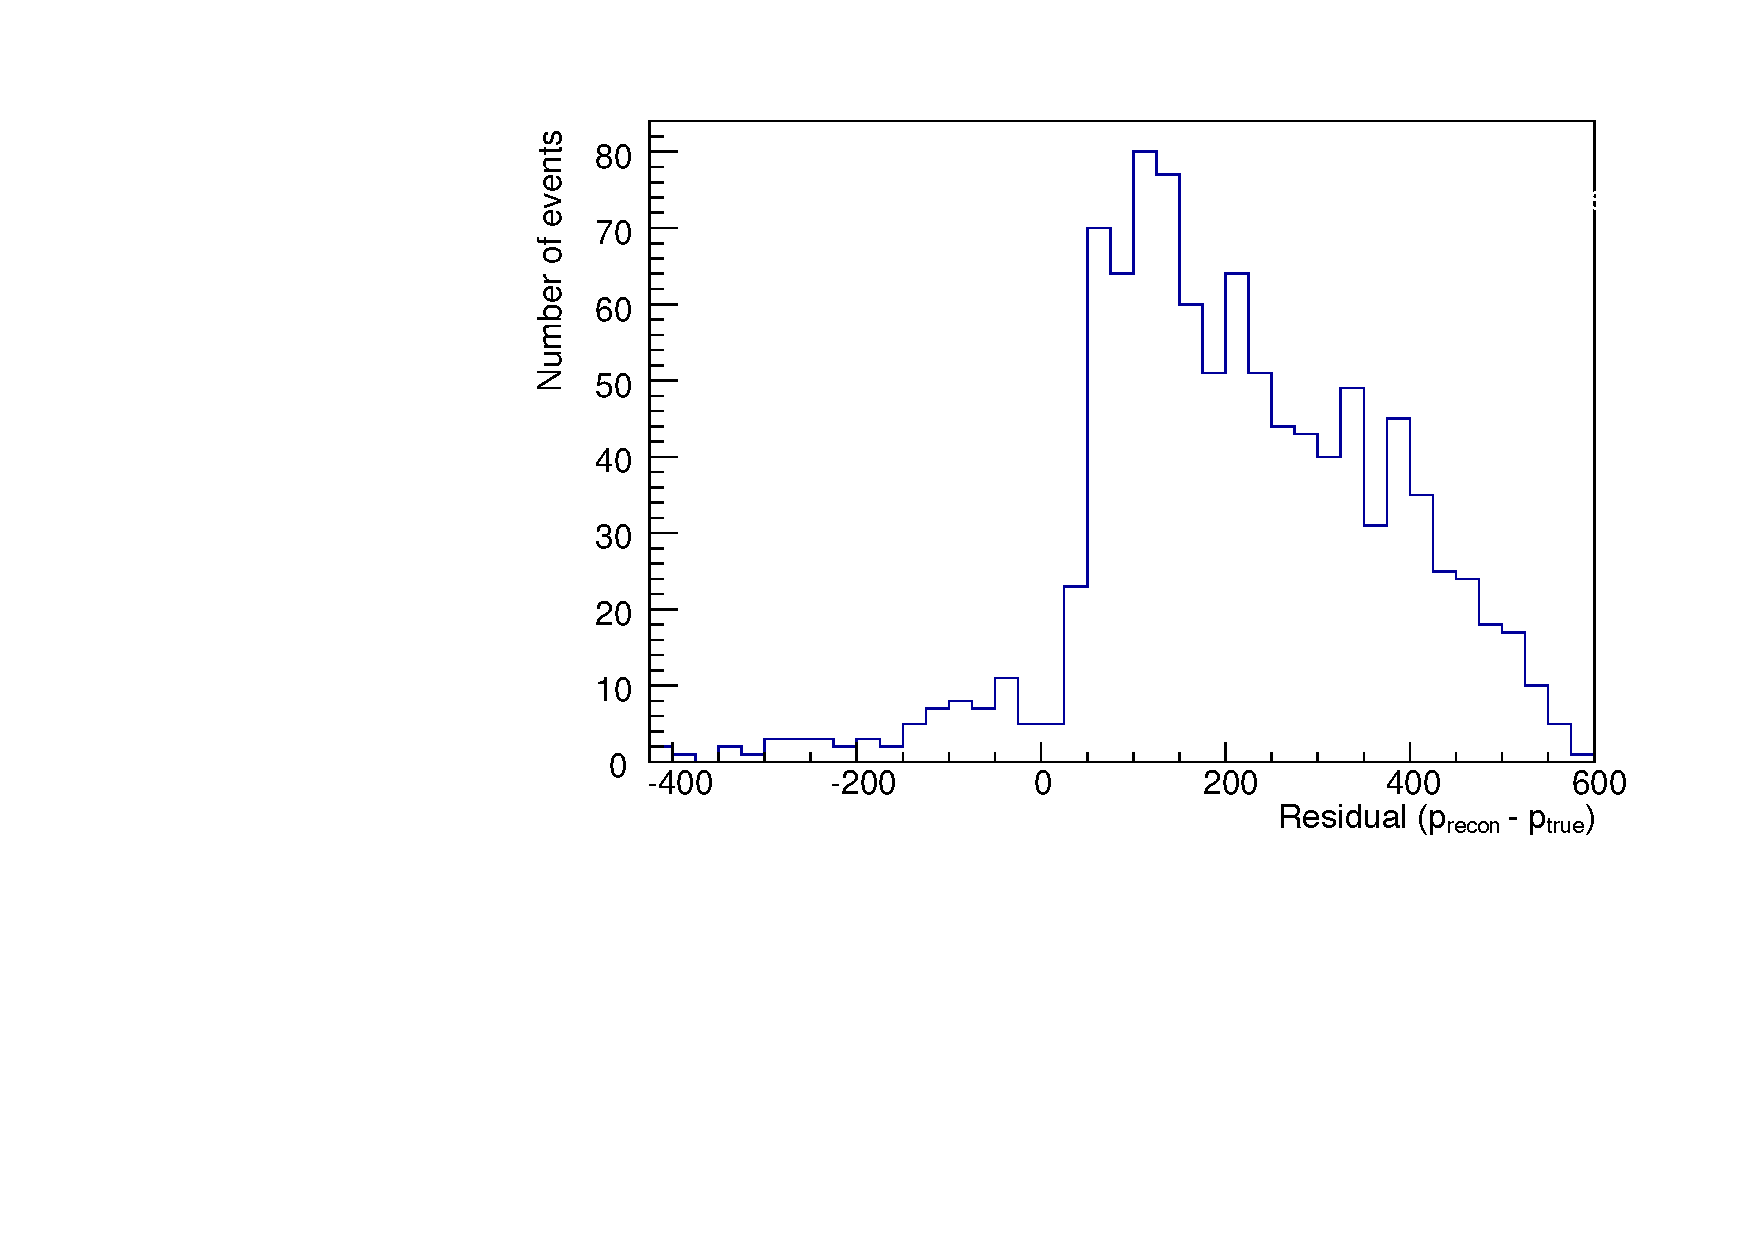
\includegraphics[angle=-90,width=\textwidth]{chapters/trackfitting_images/kalman-ccqe-low-constrained-residuals}
    \caption[Residuals for constrained momentum reconstruction at $E_\nu = 770\MeV$]{\label{fig:kalman-constrained-ccqe-770-residuals}Residuals (reconstructed momentum minus true momentum) for a Kalman filter performing a constrained momentum reconstruction of muons resulting from $770\MeV$ muon neutrinos interacting in liquid Argon and producing $\ccqe$ (only) final states. Data from $10^3$ events is shown, of which only $5$ have a residual close to zero (which indicates a perfect reconstruction). Most events have a positive residual (which indicates a tendency for the algorithm to over-estimate) and there are many events with large residuals. These results indicate that the algorithm used is not well-suited to this task, and is not capable of delivering accurate momentum estimates on data of this type.}
\end{figure}

The analysis was repeated with $10^4$ muon tracks from interactions of $4.5\GeV$ muon-neutrinos, setting the maximum momentum estimate at each step to $4.5\GeV$. The resulting distribution is shown in figure \ref{fig:kalman-constrained-ccqe-high}, where it is compared to the true distribution. The residuals are not shown, since no events were reconstructed with a momentum less than the maximum allowed by the constraints, hence this reconstruction is no better than simply assuming that each muon carries the maximum possible momentum. These results again demonstrate that the Kalman filter is unfit for the general purpose reconstruction of muon momenta in this environment.

\begin{figure}
    \centering
    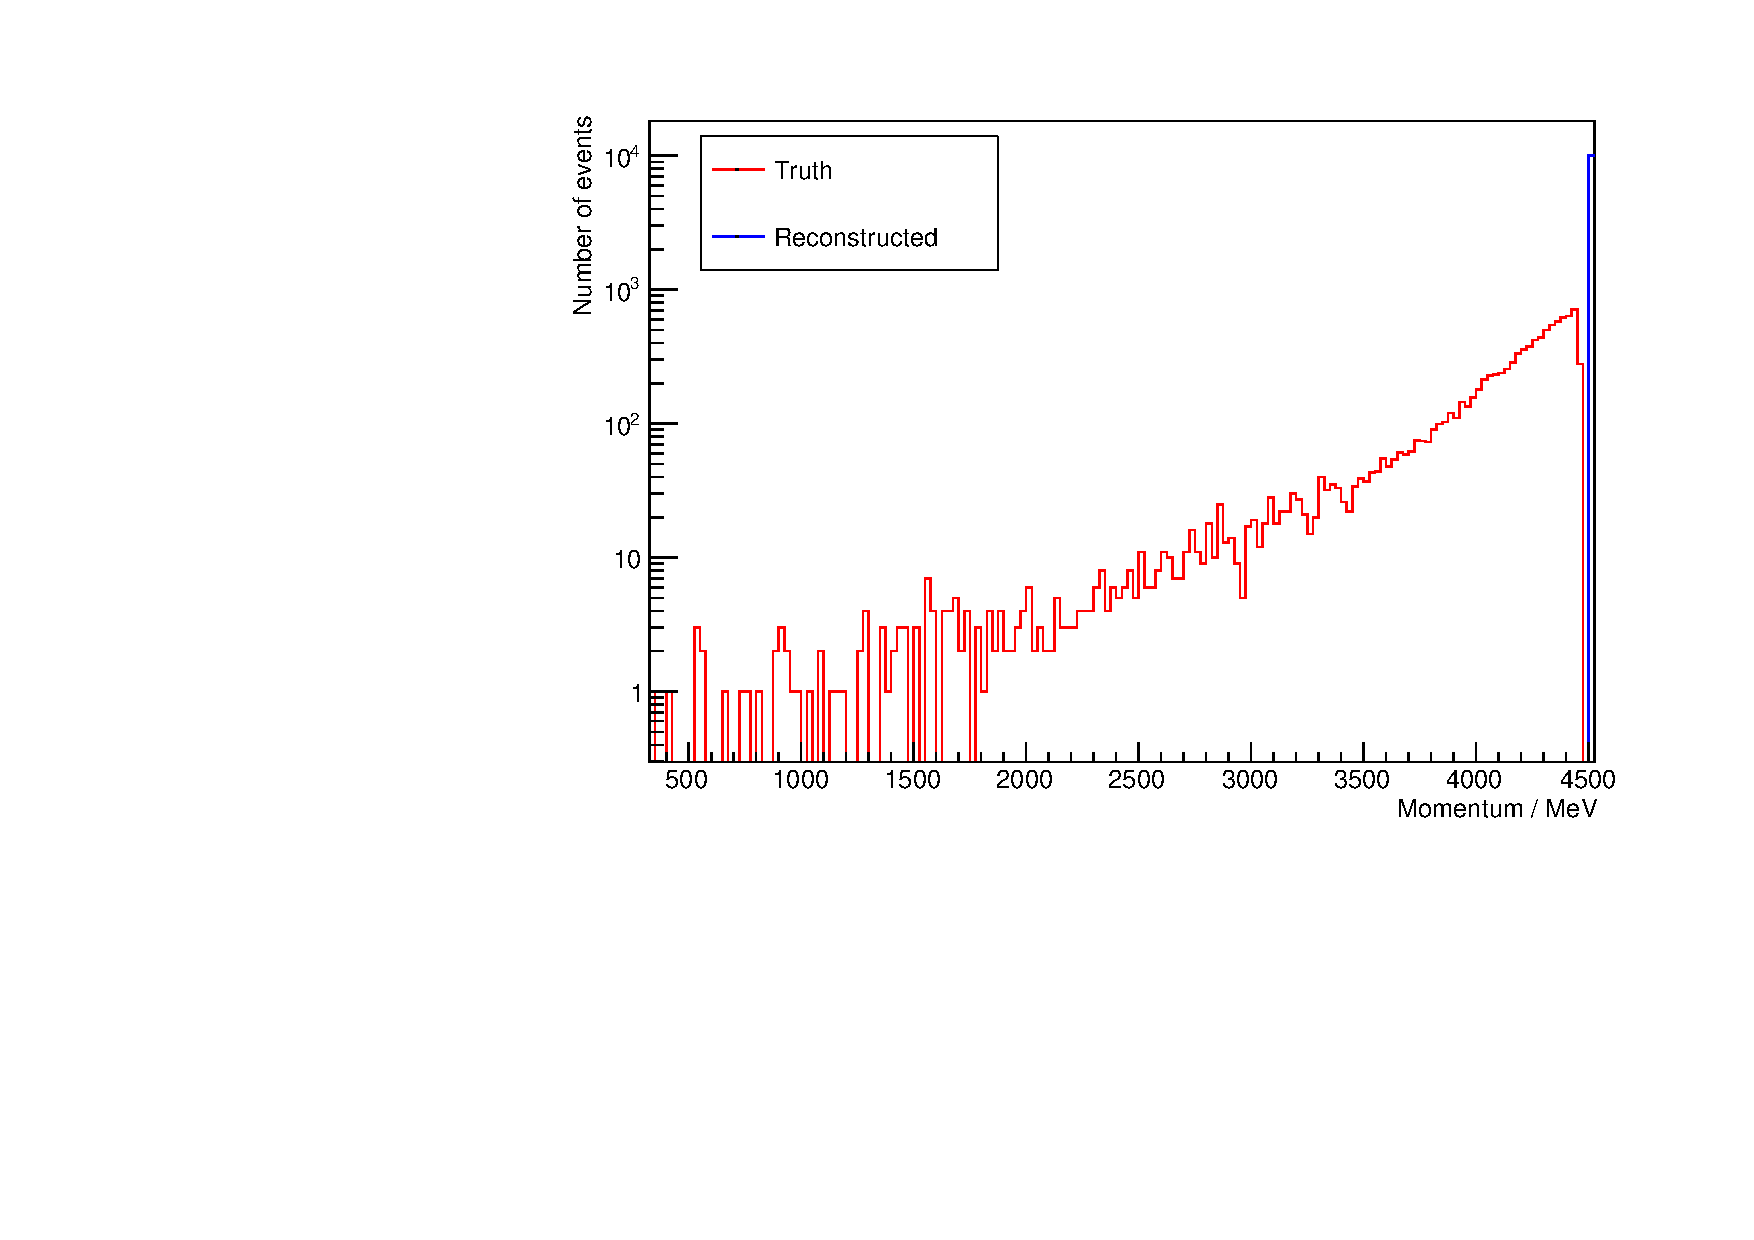
\includegraphics[angle=-90,width=\textwidth]{chapters/trackfitting_images/kalman-ccqe-high-constrained}
    \caption[True and reconstructed muon momentum distributions at $4.5\GeV$ (constrained)]{\label{fig:kalman-constrained-ccqe-high}Distribution of momenta for muons produced in a charged current $\nu_\mu$ interaction at $4.5\GeV$ resulting in a $\ccqe$ (only) final state (in red). The distribution of reconstructed momenta (in blue) is from the output of the Kalman filter applied to $10^4$ such events, with the momentum estimate at each step constrained such that $0 \le |\vec{p}| \le 4500\MeV$. The y-axis (number of events) is shown on a log scale. There is no overlap at all between the two distributions; every muon track is reconstructed with the highest allowed momentum.}
\end{figure}

\clearpage
\section{Conclusions}
The Kalman filter is traditionally a powerful tool for track parameter estimation, but in the environment of a \ac{LAr TPC} it does not perform well, at least for the estimation of track momentum. The Icarus experiment achieved better results, but with a smaller measurement error on their individual hits ($400\micron$)~\citep{Ankowski2006}. For data of the type presented here, the Kalman filter (as implemented) is not a good reconstruction tool for the purposes of estimating particle momentum. Attempts to constrain the estimates at each step of the procedure do not improve the end result and serve only as a simple `sanity check' to avoid unphysical reconstructed momenta.

The spatial track parameters were not considered here because muons in liquid Argon undergo frequent large scatters, resulting in tracks that can have substantial curvature or kinks. These track features make it extremely difficult to compare the state of the Kalman filter to the spatial parameters of the whole track, and would have to be considered on a smaller scale, with instantaneous state vectors.
